\chapter{Scelte di progetto}

\section{Java Bean}\label{sec:java_bean}
Le JavaBean sono usate per incapsulare molti oggetti in un singolo oggetto (il bean), così da poter passare il bean invece degli oggetti individuali.
Al fine di funzionare come una classe JavaBean, una classe comune di un oggetto deve obbedire a certe convenzioni in merito ai nomi, alla costruzione e al comportamento dei metodi. 
Le convenzioni richieste sono:
\begin{itemize}
    \item La classe deve avere un costruttore senza argomenti.
    \item Le sue proprietà devono essere accessibili usando get, set e altri metodi (così detti metodi accessori).
    \item La classe dovrebbe essere serializzabile (capace di salvare e ripristinare il suo stato in modo persistente).
    \item Non dovrebbe contenere alcun metodo richiesto per la gestione degli eventi.
\end{itemize}

Utilizzando queste proprietà, i Java Bean sono risultati molto utili sia per creare strutture facilmente inviabili via rete, sia per utilizzare le classi XMLEncoder e XMLDecoder per scrivere e leggere Java Bean da file XML.

\section{UML Logica}\label{sec:UML_logica}
\begin{figure}[t]
 \centering
 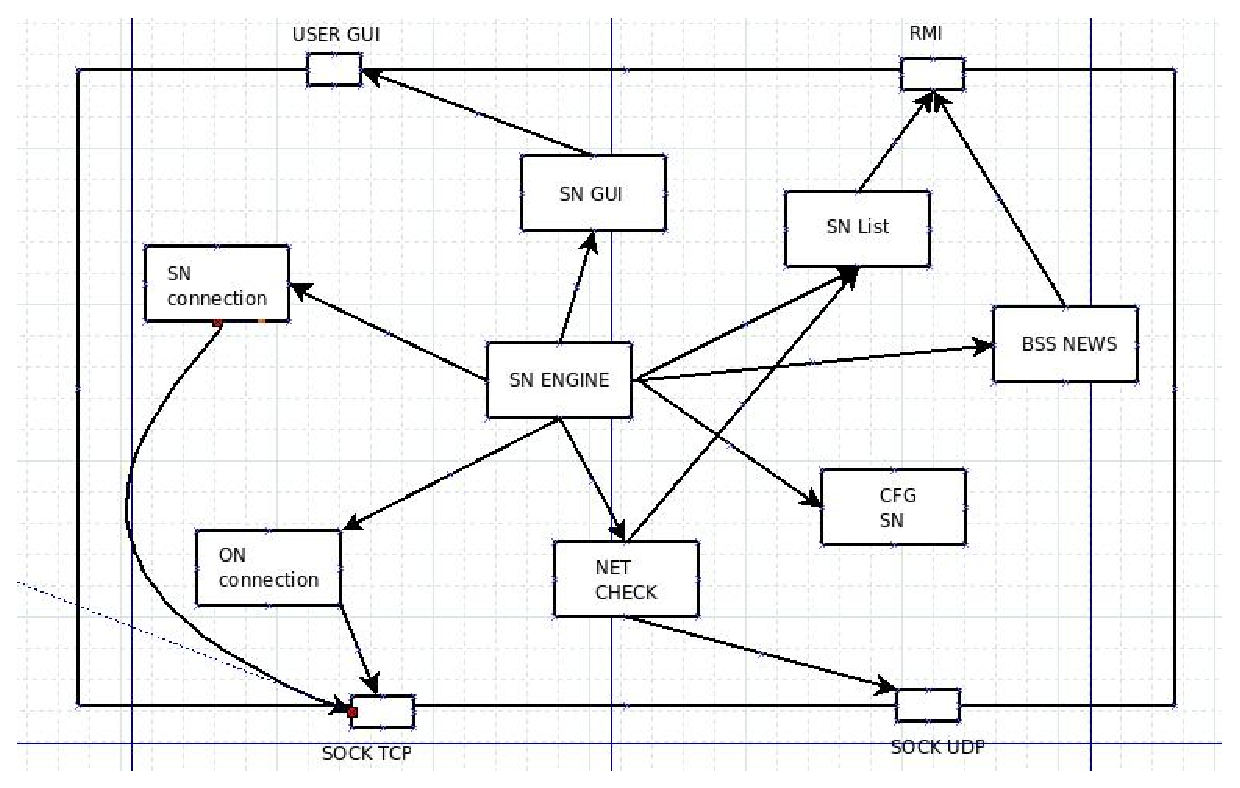
\includegraphics[width=400px,height=225px,bb=14 14 593 376]{images/logica_uml.eps}
 % logica_uml.eps: 0x0 pixel, 300dpi, 0.00x0.00 cm, bb=14 14 593 376
 \caption{Il diagramma UML che rappresenta la logica di Mini-KaZaA.}
 \label{fig:logica_uml}
\end{figure}
%Inserire una breve descrizione del diagramma UML
La logica del programma è visualizzabile in Figura \ref{fig:logica_uml}.
Il diagramma UML si riferisce un nodo di tipo SN, ma, visto che possiamo considerare i SN come degli ON con alcune funzionalità in più, questo diagramma vale anche per gli ON.

Possiamo vedere come ogni nodo abbia due tipi di componenti:
\begin{itemize}
 \item componenti logica interna;
 \item componenti di interfaccia con il mondo esterno.
\end{itemize}

Tutti questi componenti vengono gestiti da un motore centrale.


\section{Classe Wrapper per il socket}\label{sec:wrap_sock}
Il fine del Wrapper è di fornire una soluzione astratta al problema dell'interoperabilità tra interfacce differenti. Il problema si presenta ogni qual volta nel progetto di un software si debbano utilizzare sistemi di supporto (come per esempio librerie) dotati di interfaccia non perfettamente compatibile con quelle richieste da applicazioni già esistenti. Invece di dover riscrivere parte del sistema, oneroso e non sempre possibile se non si ha a disposizione il codice sorgente, può essere comodo scrivere un Adapter che faccia da tramite tra le diverse interfacce, rendendole così compatibili.
